\documentclass{article}
\usepackage{amsmath}
\usepackage{braket}
\usepackage{graphicx}
\usepackage{tikz}
\usepackage{mathtools}
\begin{document}
\section{GFN2-xTB $E^\Gamma$}
\subsection{Quantum Digital Arithmetic}
\begin{equation}
    E^\Gamma = \frac{1}{3}\sum_A\sum_{\mu\in A} (q_{A,\mu})^3\Gamma_{A,\mu}
\end{equation}
where $q_{A,\nu}=\sum_B\sum_{\nu\in B}P_{\mu\nu}S_{\mu\nu}$ is the partial charge of shell $\mu$ associated with atom $A$. $P, S$ are the density and overlap matrices. $\Gamma_{A,\mu} = \Gamma_A K_\mu$ is just the product of an element specific constant and a shell specific constant, for our purposes the element is always carbon and the shell is either the first or second in GFN2 thus we have 2 numbers $\Gamma_{\text{Carbon},0(1)}$ henceforth referred to as $\varGamma_{0(1)}$. 

\vspace{\baselineskip}
\noindent
Let us first rewrite the inner expression a bit given our new definition and knowledge of the atoms we are working with. 
\begin{equation}
    \sum_{\mu\in A} (q_{A,\mu})^3\Gamma_{A,\mu} = \sum_{\mu \in \{0,1\}} (q_{A,\mu})^3\varGamma_{\mu}
\end{equation}

We now need a unitary which computes this function on a given state $\ket{q_{A,\mu}}_Q\ket{\varGamma_\mu}_\Gamma\ket{acc}_E \to \ket{q_{A,\mu}}_Q\ket{\varGamma_\mu}_\Gamma\ket{acc+(q_{A,\mu})^3\varGamma_{\mu}}_E$. 
Consider having access to the following addition (multiplication) unitary $\ket{A}\ket{B} \to \ket{A}\ket{A+(*)B}$. 
We can now apply the following unitary ${E_i^\Gamma}_{(Q,\Gamma,E)} = \text{MULT}^{\dagger^3}_{Q,\Gamma}\text{ADD}_{\Gamma,E}\text{MULT}^{3}_{Q,\Gamma}$.  
\begin{align}
    {E_i^\Gamma}_{(Q,\Gamma,E)}&\ket{q_{A,\mu}}_Q\ket{\varGamma_\mu}_\Gamma\ket{acc}_E\\
    =\text{MULT}^{\dagger^3}_{Q,\Gamma}\text{ADD}_{\Gamma,E}\text{MULT}^{3}_{Q,\Gamma}&\ket{q_{A,\mu}}_Q\ket{\varGamma_\mu}_\Gamma\ket{acc}_E\\ 
    = \text{MULT}^{\dagger^3}_{Q,\Gamma}\text{ADD}_{\Gamma,E}\text{MULT}^{2}_{Q,\Gamma}&\ket{q_{A,\mu}}_Q\ket{q_{A,\mu}\varGamma_\mu}_\Gamma\ket{acc}_E\\
    = \text{MULT}^{\dagger^3}_{Q,\Gamma}\text{ADD}_{\Gamma,E}\text{MULT}_{Q,\Gamma}&\ket{q_{A,\mu}}_Q\ket{(q_{A,\mu})^2\varGamma_\mu}_\Gamma\ket{acc}_E\\
    = \text{MULT}^{\dagger^3}_{Q,\Gamma}\text{ADD}_{\Gamma,E}&\ket{q_{A,\mu}}_Q\ket{(q_{A,\mu})^3\varGamma_\mu}_\Gamma\ket{acc}_E\\
    = \text{MULT}^{\dagger^3}_{Q,\Gamma}&\ket{q_{A,\mu}}_Q\ket{(q_{A,\mu})^3\varGamma_\mu}_\Gamma\ket{acc+(q_{A,\mu})^3\varGamma_\mu}_E\\
    = \text{MULT}^{\dagger^2}_{Q,\Gamma}&\ket{q_{A,\mu}}_Q\ket{(q_{A,\mu})^2\varGamma_\mu}_\Gamma\ket{acc+(q_{A,\mu})^3\varGamma_\mu}_E\\
    = \text{MULT}^{\dagger}_{Q,\Gamma}&\ket{q_{A,\mu}}_Q\ket{q_{A,\mu}\varGamma_\mu}_\Gamma\ket{acc+(q_{A,\mu})^3\varGamma_\mu}_E\\
    = &\ket{q_{A,\mu}}_Q\ket{\varGamma_\mu}_\Gamma\ket{acc+(q_{A,\mu})^3\varGamma_\mu}_E\\
\end{align}
This circuit to compute the inner sum in $E^\Gamma$ could be called ${E_i^\Gamma}_{(Q,\Gamma,E)}$. Let us say we are given a circuit, SDA, for encoding a molecule from its ID in the following manner. 
\begin{equation}
\begin{split}
    \text{SDA}\ket{ID}_{ID}\ket{0}=&\\
    \ket{ID}_{ID}\ket{0}_E\ket{0}_C\ket{0}_W&\bigotimes_{A_n\in \text{Atoms}}\left(\ket{q_{A_n,0}}_{Q_{n,0}}\ket{q_{A_n,1}}_{Q_{n,1}}\right)\ket{\varGamma_0}_{\Gamma_0}\ket{\varGamma_1}_{\Gamma_1} 
\end{split}
\end{equation}
We can now apply $\text{DA}=\prod_{\mu\in\{0,1\}}\prod_{A_n} {E_i^\Gamma}_{(Q_{n,\mu},\Gamma_\mu,E)}$ to get 
\begin{equation}
\begin{split}
    \text{DA}&\ket{ID}_{ID}\ket{0}_E\ket{0}_C\ket{0}_W\bigotimes_{A_n}\left(\ket{q_{A_n,0}}_{Q_{n,0}}\ket{q_{A_n,1}}_{Q_{n,1}}\right)\ket{\varGamma_0}_{\Gamma_0}\ket{\varGamma_1}_{\Gamma_1} = \\
    &\ket{ID}_{ID}\ket{E^\Gamma}_E\ket{0}_C\ket{0}_W\bigotimes_{A_n}\left(\ket{q_{A_n,0}}_{Q_{n,0}}\ket{q_{A_n,1}}_{Q_{n,1}}\right)\ket{\varGamma_0}_{\Gamma_0}\ket{\varGamma_1}_{\Gamma_1}
\end{split}
\end{equation}

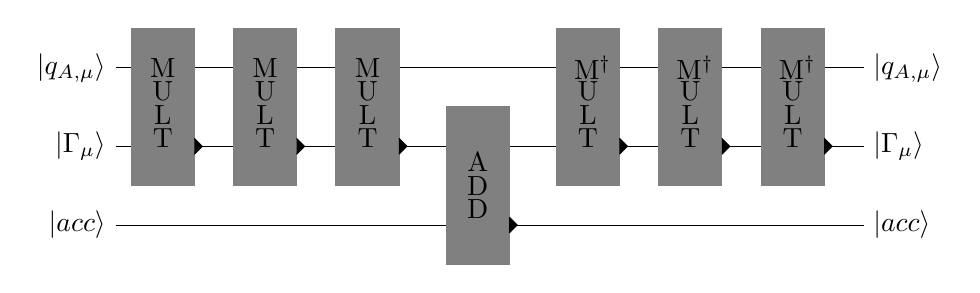
\begin{tikzpicture}[scale=1, transform shape]
    \node[rectangle,anchor=east] at (-1,2) {$\ket{q_{A,\mu}}$};
    \node[rectangle,anchor=east] at (-1,1) {$\ket{\Gamma_\mu}$};
    \node[rectangle,anchor=east] at (-1,0) {$\ket{acc}$};

    \node[rectangle,anchor=west] at ( 8.5,2) {$\ket{q_{A,\mu}}$};
    \node[rectangle,anchor=west] at ( 8.5,1) {$\ket{\Gamma_\mu}$};
    \node[rectangle,anchor=west] at ( 8.5,0) {$\ket{acc}$};
    \foreach \y in {0,...,2}
        \draw (-1,\y) -- (8.5,\y) ;
    \foreach \x in {0,...,2}{
        \filldraw[gray] (-0.8+\x*1.3+0,2.5) rectangle (0+\x*1.3,.5);
        \filldraw[black] (0+\x*1.3,.9) -- (0+\x*1.3+0.1,1) -- (0+\x*1.3,1.1);
        \node[] at (-0.4+\x*1.3+0,2.0) {M}; 
        \node[] at (-0.4+\x*1.3+0,1.7) {U}; 
        \node[] at (-0.4+\x*1.3+0,1.4) {L}; 
        \node[] at (-0.4+\x*1.3+0,1.1) {T}; 
    }
    \foreach \x in {0,...,2}{
        \filldraw[gray] (-0.8+\x*1.3+5.4,2.5) rectangle (5.4+\x*1.3,.5);
        \filldraw[black] (5.4+\x*1.3,.9) -- (5.4+\x*1.3+0.1,1) -- (5.4+\x*1.3,1.1);
        \node[anchor=west] at (-0.4+\x*1.3+5.1,2.0) {M$ ^\dagger$}; 
        \node[] at (-0.4+\x*1.3+5.4,1.7) {U}; 
        \node[] at (-0.4+\x*1.3+5.4,1.4) {L}; 
        \node[] at (-0.4+\x*1.3+5.4,1.1) {T}; 
    }

    \filldraw[gray] (3.2,1.5) rectangle (4,-.5);
    \filldraw[black] (4,-.1) -- (4.1,0) -- (4,.1);
    \node[] at (3.6,0.8) {A}; 
    \node[] at (3.6,0.5) {D}; 
    \node[] at (3.6,0.2) {D}; 
        
\end{tikzpicture}
\subsection{Sampling using Quantum Amplitude Arithmetic}
Assume that we are given an equal superposition of all the canonical IDs of the fullerenes in an isomer-space. We can apply SDA to set up the encoding and then apply $DA$. We now have computed the $E^\Gamma$ energies for every isomer. However we can only sample once! Let us say that we are interested in the isomers with the lowest energies. We then would like the probability of sampling an isomer to be proportional to $E^\Gamma$. We can achieve this using Quantum Amplitude Arithmetic, not to be confused with Quantum Amplitude Amplification, both shortened as QAA but in this writing as QA-Arithmetic and QA-Amplification. 


\vspace{\baselineskip}
The paper on QA-Arithmetic uses the introduced addition and multiplication primitives to construct a circuit which transforms the state $\ket{x}_D\ket{0}_C\ket{0}_W \to \frac{1}{2}\frac{x}{2^n}\ket{x}_D\ket{0}_C\ket{1}_W+\alpha\ket{\omega}_{D \otimes C\otimes W}$ where $\alpha$ is some normalization factor, and $\ket{\omega}$ is some state with no overlap with the state containing all 0's in the control register, $C$, and 1 in the work register, $W$.


\vspace{\baselineskip}
When using this circuit we can treat the $E$ register containing our resulting $E^\Gamma$ term as the data register, $D$. Let us take a look at that.
\begin{equation}
   \resizebox{.9\hsize}{!}{$\begin{split}
       \sum_{ID\in \text{isomers}}&\left [ \ket{ID}_{ID}\ket{E^\Gamma_{ID}}_E\ket{0}_C\ket{0}_W\bigotimes_{A_n}\left ( \ket{q_{A_n,0}}_{Q_{n,0}}\ket{q_{A_n,1}}_{Q_{n,1}}\right ) \right ] \ket{\varGamma_0}_{\Gamma_0}\ket{\varGamma_1}_{\Gamma_1} \to\\ 
        \sum_{ID\in \text{isomers}}&\left [ \ket{ID}_{ID}\left(\frac{1}{2}\frac{E^\Gamma_{ID}}{2^n}\ket{E^\Gamma_{ID}}_E\ket{0}_C\ket{1}_W+\alpha_{ID}\ket{\omega_{ID}}\right)\bigotimes_{A_n}\left ( \ket{q_{A_n,0}}_{Q_{n,0}}\ket{q_{A_n,1}}_{Q_{n,1}}\right ) \right ] \ket{\varGamma_0}_{\Gamma_0}\ket{\varGamma_1}_{\Gamma_1}\\ 
   \end{split}$}
\end{equation}
If we now sample from this superposition and postselect for $C = 0$ and $W = 1$ we are more likely to sample a low energy fullerene. The likelihood of sampling a given canonical fullerene ID is proportional with $E^\Gamma$ for that fullerene.

\subsection{An alternative circuit using exclusively Quantum Amplitude Arithmetic.}
An alternative strategy would be to go all in on QA-Arithmetic and do all the arithmetic in the amplitudes. 
Here we would encode a molecule as follows
\begin{equation}
    \text{SAA}\ket{ID}_{ID}\ket{0}_{\Gamma\otimes Q\otimes C\otimes W}=\ket{ID}_{ID}\sum_{\mu\in\{0,1\}}\ket{\varGamma_\mu}_\Gamma\sum_{A_n}\ket{q_{A_n,\mu}}_Q\ket{0}_{C}\ket{0}_{W}
\end{equation}
Where $C = C_1\otimes C_2\otimes C_3\otimes C_4$ and $W = W_1\otimes W_2\otimes W_3\otimes W_4$.
We can now apply the QA-Arithmetic papers transformation 4 times. This would be on the $(\Gamma,C_1,W_1), (Q,C_2,W_2), (Q,C_3,W_3), (Q,C_4,W_4)$ registers.
This would, if we collect all terms involving $\omega$ into one term, yield
\begin{equation}
    \alpha_{ID}\ket{\omega_{ID}}+\frac{1}{2^4}\ket{ID}\sum_{\mu\in\{0,1\}}\frac{\varGamma_\mu}{2^{n}}\ket{\varGamma_\mu}_\Gamma\sum_{A_n}\frac{q_{A_n,\mu}^3}{2^{n^3}}\ket{q_{A_n,\mu}}_Q\ket{0}_{C}\ket{1}_{W}
\end{equation}

If we apply this to a superposition of such molecule encodings and postselect on $C = 0$ and $W = 1$ we would sample a molecule with $ID$ with probability $\propto
    \sum_{\mu\in\{0,1\}}\sum_{A_n}\frac{\varGamma_\mu}{2^{n}}\frac{q_{A_n,\mu}^3}{2^{n^3}} =  \frac{E^\Gamma_{ID}}{2^{n^4}}\propto E^\Gamma_{ID}.
$
We can then compute the energy classically. 



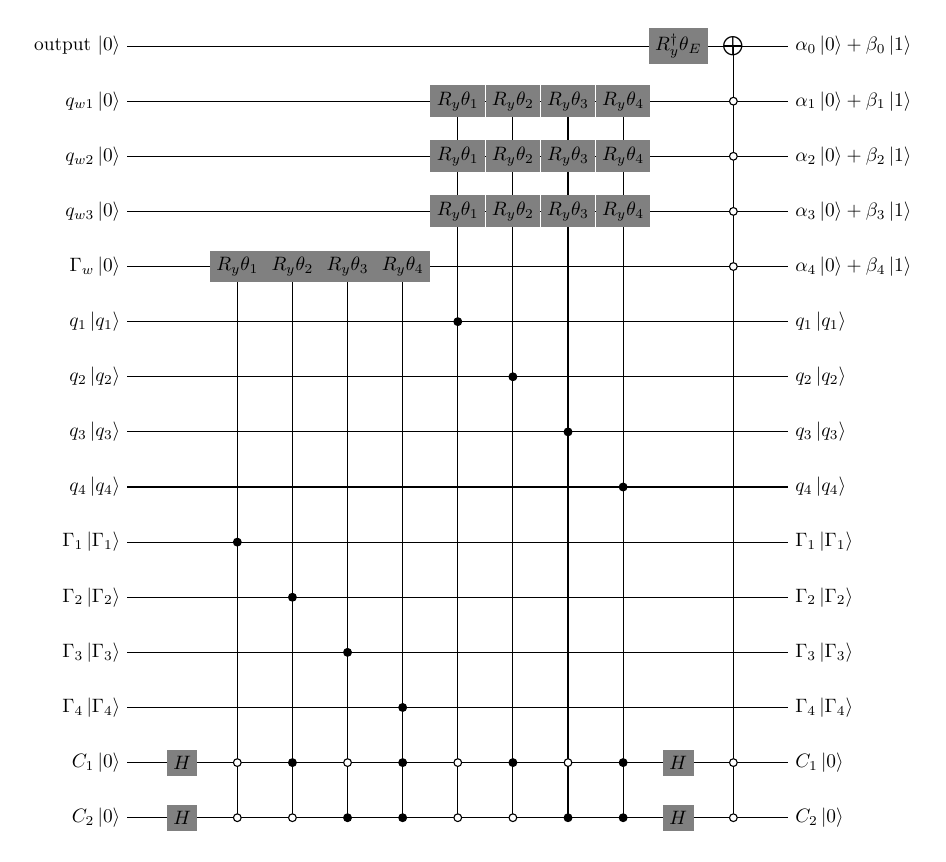
\begin{tikzpicture}[scale=0.7, transform shape]
    \node[rectangle,anchor=east] at (-1,14) {output $\ket{0}$};
    \foreach \y in {1,...,3}
        \node[rectangle,anchor=east] at (-1,14-\y) { $q_{w\y}\ket{0}$};
    \node[rectangle,anchor=east] at (-1,10) { $\Gamma_{w}\ket{0}$};

    \foreach \y in {0,...,4}
        \node[rectangle,anchor=west] at (11,14-\y) { $\alpha_{\y}\ket{0}+\beta_{\y}\ket{1}$};


    \foreach \y in {1,...,4}
        \node[rectangle,anchor=east] at (-1,10-\y) { $q_{\y}\ket{q_{\y}}$};
    \foreach \y in {1,...,4}
        \node[rectangle,anchor=east] at (-1,6-\y) { $\Gamma_{\y}\ket{\Gamma_{\y}}$};
    \foreach \y in {1,2}
        \node[rectangle,anchor=east] at (-1,2-\y) { $C_{\y}\ket{0}$};

    \foreach \y in {1,...,4}
        \node[rectangle,anchor=west] at (11,10-\y) { $q_{\y}\ket{q_{\y}}$};
    \foreach \y in {1,...,4}
        \node[rectangle,anchor=west] at (11,6-\y) { $\Gamma_{\y}\ket{\Gamma_{\y}}$};
    \foreach \y in {1,2}
        \node[rectangle,anchor=west] at (11,2-\y) { $C_{\y}\ket{0}$};

    \foreach \y in {0,...,14}
        \draw (-1,\y) -- (11,\y) ;
    \foreach \x in {1,...,4}{
        \draw (\x,0) -- (\x,10);
        \draw (\x+4,0) -- (\x+4,13);
    }
    \draw (10,0) -- (10,14);
    \node[rectangle] at (10,14) {$\bigoplus$};
    \node[rectangle,fill=gray] at (0,0) {$H$} ;
    \node[rectangle,fill=gray] at (0,1) {$H$} ;
    \node[rectangle,fill=gray] at (9,0) {$H$} ;
    \node[rectangle,fill=gray] at (9,1) {$H$} ;
    \foreach \x in {1,...,4}{
        \node[rectangle,fill=gray] at (\x,10) {$R_y\theta_\x$} ;
        \foreach \y in {11,...,13}{
            \node[rectangle,fill=gray] at (\x+4,\y) {$R_y\theta_\x$} ;
        }
    }
    \node[rectangle,fill=gray] at (9,14) {$R_y^\dagger\theta_E$} ;
    \foreach \a in {4,...,1}{
        \filldraw[black] (\a,6-\a) circle (2pt);
        \filldraw[black] (\a+4,10-\a) circle (2pt);
    }
    \foreach \y in {10,...,13}
        \filldraw[white,draw=black] (10,\y) circle (2pt);
    \foreach \x in {0,4}{
        \filldraw[black] (\x+2,1) circle (2pt);
        \filldraw[black] (\x+3,0) circle (2pt);
        \filldraw[black] (\x+4,1) circle (2pt);
        \filldraw[black] (\x+4,0) circle (2pt);
    }
    \foreach \x in {0,4}{
        \filldraw[white,draw=black] (\x+2,0) circle (2pt);
        \filldraw[white,draw=black] (\x+3,1) circle (2pt);
        \filldraw[white,draw=black] (\x+1,0) circle (2pt);
        \filldraw[white,draw=black] (\x+1,1) circle (2pt);
    }
    \filldraw[white,draw=black] (10,0) circle (2pt);
    \filldraw[white,draw=black] (10,1) circle (2pt);
\end{tikzpicture}

The controlled gate notation here is the following, $t$ is the target register and $c1,c2,c3,\dots$ are the control registers. $a,b,c,\dots$ are all $1$ except if there is a bar over the corresponding $c1,c2,c3,\dots$ in which case it is $0$. 
\begin{equation}
    \begin{split}
        CU^{c1,c2,c3,\dots}_t = (U_t-I_t)\otimes &\ket{a}\bra{a}_{c1} \otimes \ket{b}\bra{b}_{c2} \otimes \ket{c}\bra{c}_{c3}\otimes\dots+\\ 
        \sum_{\alpha,\beta,\zeta,\dots\in\{0,1\}}I_t\otimes &\ket{\alpha}\bra{\alpha}_{c1} \otimes \ket{\beta}\bra{\beta}_{c2} \otimes \ket{\zeta}\bra{\zeta}_{c3}\otimes\dots. 
    \end{split}
\end{equation}
Let us follow the execution of the above diagram.
We neglect writing out the $q_{1,2,3,4},\Gamma_{1,2,3,4}$ as they never change throughout the calculation, we also neglect the $ _{o,output}$ registers for now.
We begin by applying the Hadamard gates.
\begin{equation}
    \begin{split}
        H_{C1}H_{C2}&\ket{0000}_{q_{w(1,2,3)},\Gamma_w}\ket{ 00}_{C_{(1,2)}}\to\\
        \frac{1}{2}(
        &\ket{0000}_{q_{w(1,2,3)},\Gamma_w}\ket{ 00}_{C_{(1,2)}}+\\
        &\ket{0000}_{q_{w(1,2,3)},\Gamma_w}\ket{ 01}_{C_{(1,2)}}+\\
        &\ket{0000}_{q_{w(1,2,3)},\Gamma_w}\ket{ 10}_{C_{(1,2)}}+\\
        &\ket{0000}_{q_{w(1,2,3)},\Gamma_w}\ket{ 11}_{C_{(1,2)}}
        )
    \end{split}
\end{equation}
We then apply the conditional rotation gates to some register like $\Gamma_w$ we do the following
\begin{equation}
    \begin{split}
        CRy_{\Gamma_w}^{\Gamma_4,C_1,C_2}(2\theta_4)CRy_{\Gamma_w}^{\Gamma_3,\bar{C_1},C_2}(2\theta_3)CRy_{\Gamma_w}^{\Gamma_2,C_1,\bar{C_2}}(2\theta_2)&CRy_{\Gamma_w}^{\Gamma_1,\bar{C_1},\bar{C_2}}(2\theta_1)\\
        \frac{1}{2}\sum_{x_1,x_2\in\{0,1\}}\ket{0000}_{q_{w(1,2,3)},\Gamma_w}&\ket{ x_1x_2}_{C_{(1,2)}}\to\\
        \frac{1}{2}(
        CRy_{\Gamma_w}^{\Gamma_1}(2\theta_1)\ket{0000}_{q_{w(1,2,3)},\Gamma_w}&\ket{ 00}_{C_{(1,2)}}+\\
        CRy_{\Gamma_w}^{\Gamma_2}(2\theta_2)\ket{0000}_{q_{w(1,2,3)},\Gamma_w}&\ket{ 01}_{C_{(1,2)}}+\\
        CRy_{\Gamma_w}^{\Gamma_3}(2\theta_3)\ket{0000}_{q_{w(1,2,3)},\Gamma_w}&\ket{ 10}_{C_{(1,2)}}+\\
        CRy_{\Gamma_w}^{\Gamma_4}(2\theta_4)\ket{0000}_{q_{w(1,2,3)},\Gamma_w}&\ket{ 11}_{C_{(1,2)}})\to\\
        \frac{1}{2}(
        \ket{000}[\Gamma1(cos\theta_1\ket{0}+sin\theta_1\ket{1})+(1-\Gamma_1)\ket{0}]_{q_{w(1,2,3)},\Gamma_w}&\ket{ 00}+\\
        \ket{000}[\Gamma2(cos\theta_2\ket{0}+sin\theta_2\ket{1})+(1-\Gamma_2)\ket{0}]_{q_{w(1,2,3)},\Gamma_w}&\ket{ 01}+\\
        \ket{000}[\Gamma3(cos\theta_3\ket{0}+sin\theta_3\ket{1})+(1-\Gamma_3)\ket{0}]_{q_{w(1,2,3)},\Gamma_w}&\ket{ 10}+\\
        \ket{000}[\Gamma4(cos\theta_4\ket{0}+sin\theta_4\ket{1})+(1-\Gamma_4)\ket{0}]_{q_{w(1,2,3)},\Gamma_w}&\ket{ 11}
        )
    \end{split}
\end{equation}
Let us adopt the notation $\ket{\Psi^t_i}=t(cos\theta_i\ket{0}+sin\theta_i\ket{1})+(1-t)\ket{0}$ before redoing the application using our new notation. We also apply the rotation gates for the $q_w$ registers:
\begin{equation}
    \begin{split}
        CRy_{\Gamma_w}^{\Gamma_4,C_1,C_2}(2\theta_4)CRy_{\Gamma_w}^{\Gamma_3,\bar{C_1},C_2}(2\theta_3)CRy_{\Gamma_w}^{\Gamma_2,C_1,\bar{C_2}}(2\theta_2)&CRy_{\Gamma_w}^{\Gamma_1,\bar{C_1},\bar{C_2}}(2\theta_1)\\
        CRy_{q_{w1}}^{q_4,C_1,C_2}(2\theta_4)CRy_{q_{w1}}^{q_3,\bar{C_1},C_2}(2\theta_3)CRy_{q_{w1}}^{q_2,C_1,\bar{C_2}}(2\theta_2)&CRy_{q_{w1}}^{q_1,\bar{C_1},\bar{C_2}}(2\theta_1)\\
        CRy_{q_{w2}}^{q_4,C_1,C_2}(2\theta_4)CRy_{q_{w2}}^{q_3,\bar{C_1},C_2}(2\theta_3)CRy_{q_{w2}}^{q_2,C_1,\bar{C_2}}(2\theta_2)&CRy_{q_{w2}}^{q_1,\bar{C_1},\bar{C_2}}(2\theta_1)\\
        CRy_{q_{w3}}^{q_4,C_1,C_2}(2\theta_4)CRy_{q_{w3}}^{q_3,\bar{C_1},C_2}(2\theta_3)CRy_{q_{w3}}^{q_2,C_1,\bar{C_2}}(2\theta_2)&CRy_{q_{w3}}^{q_1,\bar{C_1},\bar{C_2}}(2\theta_1)\\
        \frac{1}{2}\sum_{x_1,x_2\in\{0,1\}}\ket{0000}_{q_{w(1,2,3)},\Gamma_w}&\ket{ x_1x_2}=\\
        \frac{1}{2}(
        CRy_{q_{w1}}^{q_1}(2\theta_1)CRy_{q_{w2}}^{q_1}(2\theta_1)CRy_{q_{w3}}^{q_1}(2\theta_1) CRy_{\Gamma_w}^{\Gamma_1}(2\theta_1)&\ket{0000}_{q_{w(1,2,3)},\Gamma_w}\ket{ 00}+\\
        CRy_{q_{w1}}^{q_2}(2\theta_2)CRy_{q_{w2}}^{q_2}(2\theta_2)CRy_{q_{w3}}^{q_2}(2\theta_2) CRy_{\Gamma_w}^{\Gamma_2}(2\theta_2)&\ket{0000}_{q_{w(1,2,3)},\Gamma_w}\ket{ 01}+\\
        CRy_{q_{w1}}^{q_3}(2\theta_3)CRy_{q_{w2}}^{q_3}(2\theta_3)CRy_{q_{w3}}^{q_3}(2\theta_3) CRy_{\Gamma_w}^{\Gamma_3}(2\theta_3)&\ket{0000}_{q_{w(1,2,3)},\Gamma_w}\ket{ 10}+\\
        CRy_{q_{w1}}^{q_4}(2\theta_4)CRy_{q_{w2}}^{q_4}(2\theta_4)CRy_{q_{w3}}^{q_4}(2\theta_4) CRy_{\Gamma_w}^{\Gamma_4}(2\theta_4)&\ket{0000}_{q_{w(1,2,3)},\Gamma_w}\ket{ 11})\to\\
        \frac{1}{2}(
        \ket{\Psi^{q_1}_1\Psi^{q_1}_1\Psi^{q_1}_1\Psi^{\Gamma_1}_1}_{q_{w(1,2,3)},\Gamma_w}&\ket{ 00}+\\
        \ket{\Psi^{q_2}_2\Psi^{q_2}_2\Psi^{q_2}_2\Psi^{\Gamma_2}_2}_{q_{w(1,2,3)},\Gamma_w}&\ket{ 01}+\\
        \ket{\Psi^{q_3}_3\Psi^{q_3}_3\Psi^{q_3}_3\Psi^{\Gamma_3}_3}_{q_{w(1,2,3)},\Gamma_w}&\ket{ 10}+\\
        \ket{\Psi^{q_4}_4\Psi^{q_4}_4\Psi^{q_4}_4\Psi^{\Gamma_4}_4}_{q_{w(1,2,3)},\Gamma_w}&\ket{ 11}
        )
    \end{split}
\end{equation}
Let us now apply the second set of Hadamard:
\begin{equation}
    \begin{split}
        H_{C_1}H_{C_2}\frac{1}{2}(
        &\ket{\Psi^{q_1}_1\Psi^{q_1}_1\Psi^{q_1}_1\Psi^{\Gamma_1}_1 }\ket{00}+\\
        &\ket{\Psi^{q_2}_2\Psi^{q_2}_2\Psi^{q_2}_2\Psi^{\Gamma_2}_2 }\ket{01}+\\
        &\ket{\Psi^{q_3}_3\Psi^{q_3}_3\Psi^{q_3}_3\Psi^{\Gamma_3}_3 }\ket{10}+\\
        &\ket{\Psi^{q_4}_4\Psi^{q_4}_4\Psi^{q_4}_4\Psi^{\Gamma_4}_4 }\ket{11}
        )\to\\
        \frac{1}{4}(
            &\ket{\Psi^{q_1}_1\Psi^{q_1}_1\Psi^{q_1}_1\Psi^{\Gamma_1}_1 }[\ket{00}+
            \ket{01}+
            \ket{10}+
            \ket{11}]+\\
            &\ket{\Psi^{q_2}_2\Psi^{q_2}_2\Psi^{q_2}_2\Psi^{\Gamma_2}_2 }[\ket{00}-
            \ket{01}+
            \ket{10}-
            \ket{11}]+\\
            &\ket{\Psi^{q_3}_3\Psi^{q_3}_3\Psi^{q_3}_3\Psi^{\Gamma_3}_3 }[\ket{00}+
            \ket{01}-
            \ket{10}-
            \ket{11}]+\\
            &\ket{\Psi^{q_4}_4\Psi^{q_4}_4\Psi^{q_4}_4\Psi^{\Gamma_4}_4 }[\ket{00}-
            \ket{01}-
            \ket{10}+
            \ket{11}]
    ) =\\ 
        \frac{1}{4}&\left[\ket{\Psi^{q_1}_1\Psi^{q_1}_1\Psi^{q_1}_1\Psi^{\Gamma_1}_1 }+\ket{\Psi^{q_2}_2\Psi^{q_2}_2\Psi^{q_2}_2\Psi^{\Gamma_2}_2 }+\ket{\Psi^{q_3}_3\Psi^{q_3}_3\Psi^{q_3}_3\Psi^{\Gamma_3}_3 }+\ket{\Psi^{q_4}_4\Psi^{q_4}_4\Psi^{q_4}_4\Psi^{\Gamma_4}_4 }\right]\ket{00}+\\
    \frac{1}{4}\bigg(&\left[\ket{\Psi^{q_1}_1\Psi^{q_1}_1\Psi^{q_1}_1\Psi^{\Gamma_1}_1 }-\ket{\Psi^{q_2}_2\Psi^{q_2}_2\Psi^{q_2}_2\Psi^{\Gamma_2}_2 }+\ket{\Psi^{q_3}_3\Psi^{q_3}_3\Psi^{q_3}_3\Psi^{\Gamma_3}_3 }-\ket{\Psi^{q_4}_4\Psi^{q_4}_4\Psi^{q_4}_4\Psi^{\Gamma_4}_4 }\right]\ket{01}+\\
        &\left[\ket{\Psi^{q_1}_1\Psi^{q_1}_1\Psi^{q_1}_1\Psi^{\Gamma_1}_1 }+\ket{\Psi^{q_2}_2\Psi^{q_2}_2\Psi^{q_2}_2\Psi^{\Gamma_2}_2 }-\ket{\Psi^{q_3}_3\Psi^{q_3}_3\Psi^{q_3}_3\Psi^{\Gamma_3}_3 }-\ket{\Psi^{q_4}_4\Psi^{q_4}_4\Psi^{q_4}_4\Psi^{\Gamma_4}_4 }\right]\ket{10}+\\
        &\left[\ket{\Psi^{q_1}_1\Psi^{q_1}_1\Psi^{q_1}_1\Psi^{\Gamma_1}_1 }-\ket{\Psi^{q_2}_2\Psi^{q_2}_2\Psi^{q_2}_2\Psi^{\Gamma_2}_2 }-\ket{\Psi^{q_3}_3\Psi^{q_3}_3\Psi^{q_3}_3\Psi^{\Gamma_3}_3 }+\ket{\Psi^{q_4}_4\Psi^{q_4}_4\Psi^{q_4}_4\Psi^{\Gamma_4}_4 }\right]\ket{11}
    \bigg) \\= 
        \frac{1}{4}&\left[\ket{\Psi^{q_1}_1\Psi^{q_1}_1\Psi^{q_1}_1\Psi^{\Gamma_1}_1 }+\ket{\Psi^{q_2}_2\Psi^{q_2}_2\Psi^{q_2}_2\Psi^{\Gamma_2}_2 }+\ket{\Psi^{q_3}_3\Psi^{q_3}_3\Psi^{q_3}_3\Psi^{\Gamma_3}_3 }+\ket{\Psi^{q_4}_4\Psi^{q_4}_4\Psi^{q_4}_4\Psi^{\Gamma_4}_4 }\right]\ket{00}+\ket{M}\\=&\ket{N}+\ket{M}
    \end{split}
\end{equation}
Before the next step let us define:
\begin{align}
    q_{cos} =& q_1cos\theta_1+q_2cos\theta_2+q_3cos\theta_3+q_4cos\theta_4+4-q_1-q_2-q_3-q_4\\
    q_{sin} =& q_1sin\theta_1+q_2sin\theta_2+q_3sin\theta_3+q_4sin\theta_4\\
    \Gamma_{cos} =& \Gamma_1cos\theta_1+\Gamma_2cos\theta_2+\Gamma_3cos\theta_3+\Gamma_4cos\theta_4+4-\Gamma_1-\Gamma_2-\Gamma_3-\Gamma_4\\
    \Gamma_{sin} =& \Gamma_1sin\theta_1+\Gamma_2sin\theta_2+\Gamma_3sin\theta_3+\Gamma_4sin\theta_4\\
    E_{sin} =& \Gamma_{sin}(q_{sin})^3\\
    \begin{split}
        E_{other} = &\Gamma_{cos}(q_{cos}^3+3q_{cos}^2q_{sin}+3q_{cos}q_{sin}^2+q_{sin}^3)\\
        &+\Gamma_{sin}(q_{cos}^3+3q_{cos}^2q_{sin}+3q_{cos}q_{sin}^2)
    \end{split}
\end{align}
Let us now add in the $ _o$ registers and apply our conditional not gates:
\begin{equation}
    \begin{split}
        &CX_{E_o}^{q_{o1},q_{o2},q_{o3},\Gamma_o}CX_{q_{o1}}^{q_{w1},\bar{C_1},\bar{C_2}}CX_{q_{o2}}^{q_{w2},\bar{C_1},\bar{C_2}}CX_{q_{o3}}^{q_{w3},\bar{C_1},\bar{C_2}}CX_{\Gamma_o}^{\Gamma_w,\bar{C_1},\bar{C_2}}\\
        &\ket{00000}_{E_o,q_{o(1,2,3)},\Gamma_o}(\ket{N}+\ket{M})=\\
        &CX_{E_o}^{q_{o1},q_{o2},q_{o3},\Gamma_o}CX_{q_{o1}}^{q_{w1}}CX_{q_{o2}}^{q_{w2}}CX_{q_{o3}}^{q_{w3}}CX_{\Gamma_o}^{\Gamma_w}
        \ket{00000}\ket{N}+\ket{00000}\ket{M}\to\\
        &\big[E_{other}\ket{0}+E_{sin}\ket{1}\big]_{E_o}\big[q_{cos}\ket{0}+q_{sin}\ket{1}\big]_{q_{o1}}
        \big[q_{cos}\ket{0}+q_{sin}\ket{1}\big]_{q_{o2}}\\
        &\big[q_{cos}\ket{0}+q_{sin}\ket{1}\big]_{q_{o3}}\big[\Gamma_{cos}\ket{0}+\Gamma_{sin}\ket{1}\big]_{\Gamma_{o}}\ket{N}+
        \ket{00000}\ket{M}\\
    \end{split}
\end{equation}
After applying those gates we see that the amplitude on $\ket{1}_{E_o}$ across the whole state is $\frac{1}{4}E_{sin}=(\Gamma_1sin\theta_1+\Gamma_2sin\theta_2+\Gamma_3sin\theta_3+\Gamma_4sin\theta_4)(q_1sin\theta_1+q_2sin\theta_2+q_3sin\theta_3+q_4sin\theta_4)^3$.
If we specify $\theta_i=arcsin\frac{1}{2^i}$ we get that $\frac{1}{4}E_{sin}=\frac{1}{4}(\frac{\Gamma_1}{2}+\frac{\Gamma_2}{2^2}+\frac{\Gamma_3}{2^3}+\frac{\Gamma_4}{2^8})(\frac{q_1}{2}+\frac{q_2}{2^2}+\frac{q_3}{2^3}+\frac{q_4}{2^8})^3=\frac{1}{4}(0b0.\Gamma_1\Gamma_2\Gamma_3\Gamma_4)(0b0.q_1q_2q_3q_4)^3$. This is proportional to $E^\Gamma$! 
\subsection{Complexity}
The second algorithm has, in terms of big O notation, the same complexity as the state preparation introduced in the QA-Arithmetic paper, as it is simply 4 applications of this circuit. The state preparation can be achieved using $O(\log n)$ extra qubits and $O(n\log n)$ Toffoli gates where $n$ is the number of bits used to represent $\varGamma_\mu, q_{A_n,\mu}$. Thus if we have a $m$ bit canonical fullerene ID we end up using on the order of $m+2n+4O(\log n)=O(n+m)$ qubits and $4O(n \log n)=O(n \log n)$ Toffoli gates. 

The first circuit on the other hand uses 4 mulitplication circuits, 2 squaring circuits which could just as well be multiplication circuits and an addition circuit. A QFT addition (multiplication) circuit uses $O(n^{2(3)})$ gates and no additional qubits. Thus if we have encoded $\varGamma_{\mu},q_{A_n,\mu}, \mu \in \{0,..,l\}, A_n \in \{0,..,o\}$ each using $n$ bits we will need to perform $6lo$ multiplications and $lo$ additions, resulting in $6lo\cdot O(n^3)+lo\cdot O(n^2)=O(lon^3)$ gates, on $m+n+nl+lon = O(m+lon)$ qubits.
Additionally we then have to run the state preparation circuit which adds $O(\log n)$ qubits and $O(n\log n)$ gates, however that is not enough to change the asymptotic runtime further. 

\subsection{Cleaning up $\omega$}
We would like to get rid of the $\ket{\omega}$ term in both algorithms to avoid having to post select.
We can achieve this with amplitude amplification. 
To do amplitude amplification we first need to define what a 'good' state is, in our case we know all good states have $\ket{0}_C\ket{1}_W$. 
Second we need an oracle in terms of a unitary which flips the sign of the good state, i.e. reflecting the state around the bad state, this would be $I-2\ket{0}_C\bra{0}_C\ket{1}_W\bra{1}_W$, which can be easily implemented with controlled rotations. 
We also need a circuit which would reflect around the initial state by flipping the sign of it, given that we have a circuit $U$ for preparing the initial state that would be $I-2U\ket{0}\bra{0}U^\dagger$.
In our case the angle between the bad and initial states are $\theta_{DA} = arcsin(\frac{1}{2}\frac{E^\Gamma}{2^n}),\theta_{AA} = arcsin(\frac{1}{2^4}\frac{E^\Gamma}{2^{n4}})$ for the two algorithms. We have to do $\lfloor\frac{\pi}{4\theta}\rfloor$ repetitions to maximize the probability of measuring a good state.%Todo: fix every calculation and number in this. the propably all wrong 
\subsection{Concentrating the probabilities on the best candidates}
We now have a superposition where the probability of sampling a fullerene is proportional to the energy of that fullerene.
But is that ideal? The energies might be quite close to each other in absolute terms.
Therefore we would like to exaggerate the difference between them and then sample according to that difference.
If we knew what the highest energy was we could just subtract that from every energy calculation thus getting probabilities proportional to how much lower an energy we are working with.
Another option is if we expect the energies to be within $100(1-x)\%$ we could subtract $ex$ from every energy calculation where $e$ is the energy from a random fullerene in the isomer-space.
This is of cause not as good but quite achievable. In both algorithms we can encode $ex$ in a register and then use a digital subtraction or do a QAA state preparation addition but with all the $R_y$ gates inverted, resulting in a counter-clockwise rotation, in effect subtracting $ex$.
%Note: the following is dumb, we don't want to invert the probabilities! 
%If we expect the results from these shifted energy calculations to be in the interval $]0,1[$ we can exaggerate them further by taking the reciprocal. 
\subsection{Discussion}
From the asymptotic resource use the second algorithm is clearly superior, even if some of the multiplications and additions can be run in parallel in the first one. We do have a factor 8 lower chance of getting a useful state out, but this again does not change the asymptotics, as we can just repeat it. 
QA-Amplification might be possible since we have a very clear "good" state in both algorithms. This would reduce the need for postselection and repetitions. Preparing the initial encoding of the isomer space seems less straight forwards in the second approach than in the first unfortunately. 




\end{document}
